\documentclass[conference]{IEEEtran}
%\renewcommand{\thesubsection}{\thesection.\alph{subsection}}

%\addtolength{\oddsidemargin}{-.875in}
%\addtolength{\evensidemargin}{-.875in}
%\addtolength{\textwidth}{1.75in}
%\addtolength{\topmargin}{-.875in}
%\addtolength{\textheight}{1.75in}
	
\usepackage{bm}
\usepackage{amsmath}
\usepackage{amssymb}
\usepackage{tikz}
\usetikzlibrary{automata,positioning}
\usepackage{url}
\usepackage{float}
\usepackage{setspace}
%\usepackage{IEEEtran}
\usepackage{filecontents,lipsum}
\usepackage[noadjust]{cite}

\begin{document}
%\raggedright
%\doublespacing

\title{Week 1 Journal}
\author{Rodger Byrd}
\maketitle

%summary info here

\section{Course Goals}
My primary goal for this course are to determine whether I want to pusue a Doctor of Philosophy degree. My other goals include determining whether I'm interested in reasearch, and I would particularly like to learn how to analyze data and show statistical relevance to support a hypothesis. I'd like to learn what kind of tests you can perform on the data to support your hypothesis. I'm studying Computer Science and this will be the last class I take for my master's degree. I completed my undergraduate studies in Electrical Engineering, but I've mostly worked in the fields of software development and cyber security.
\begin{figure}[H]
  \centerline{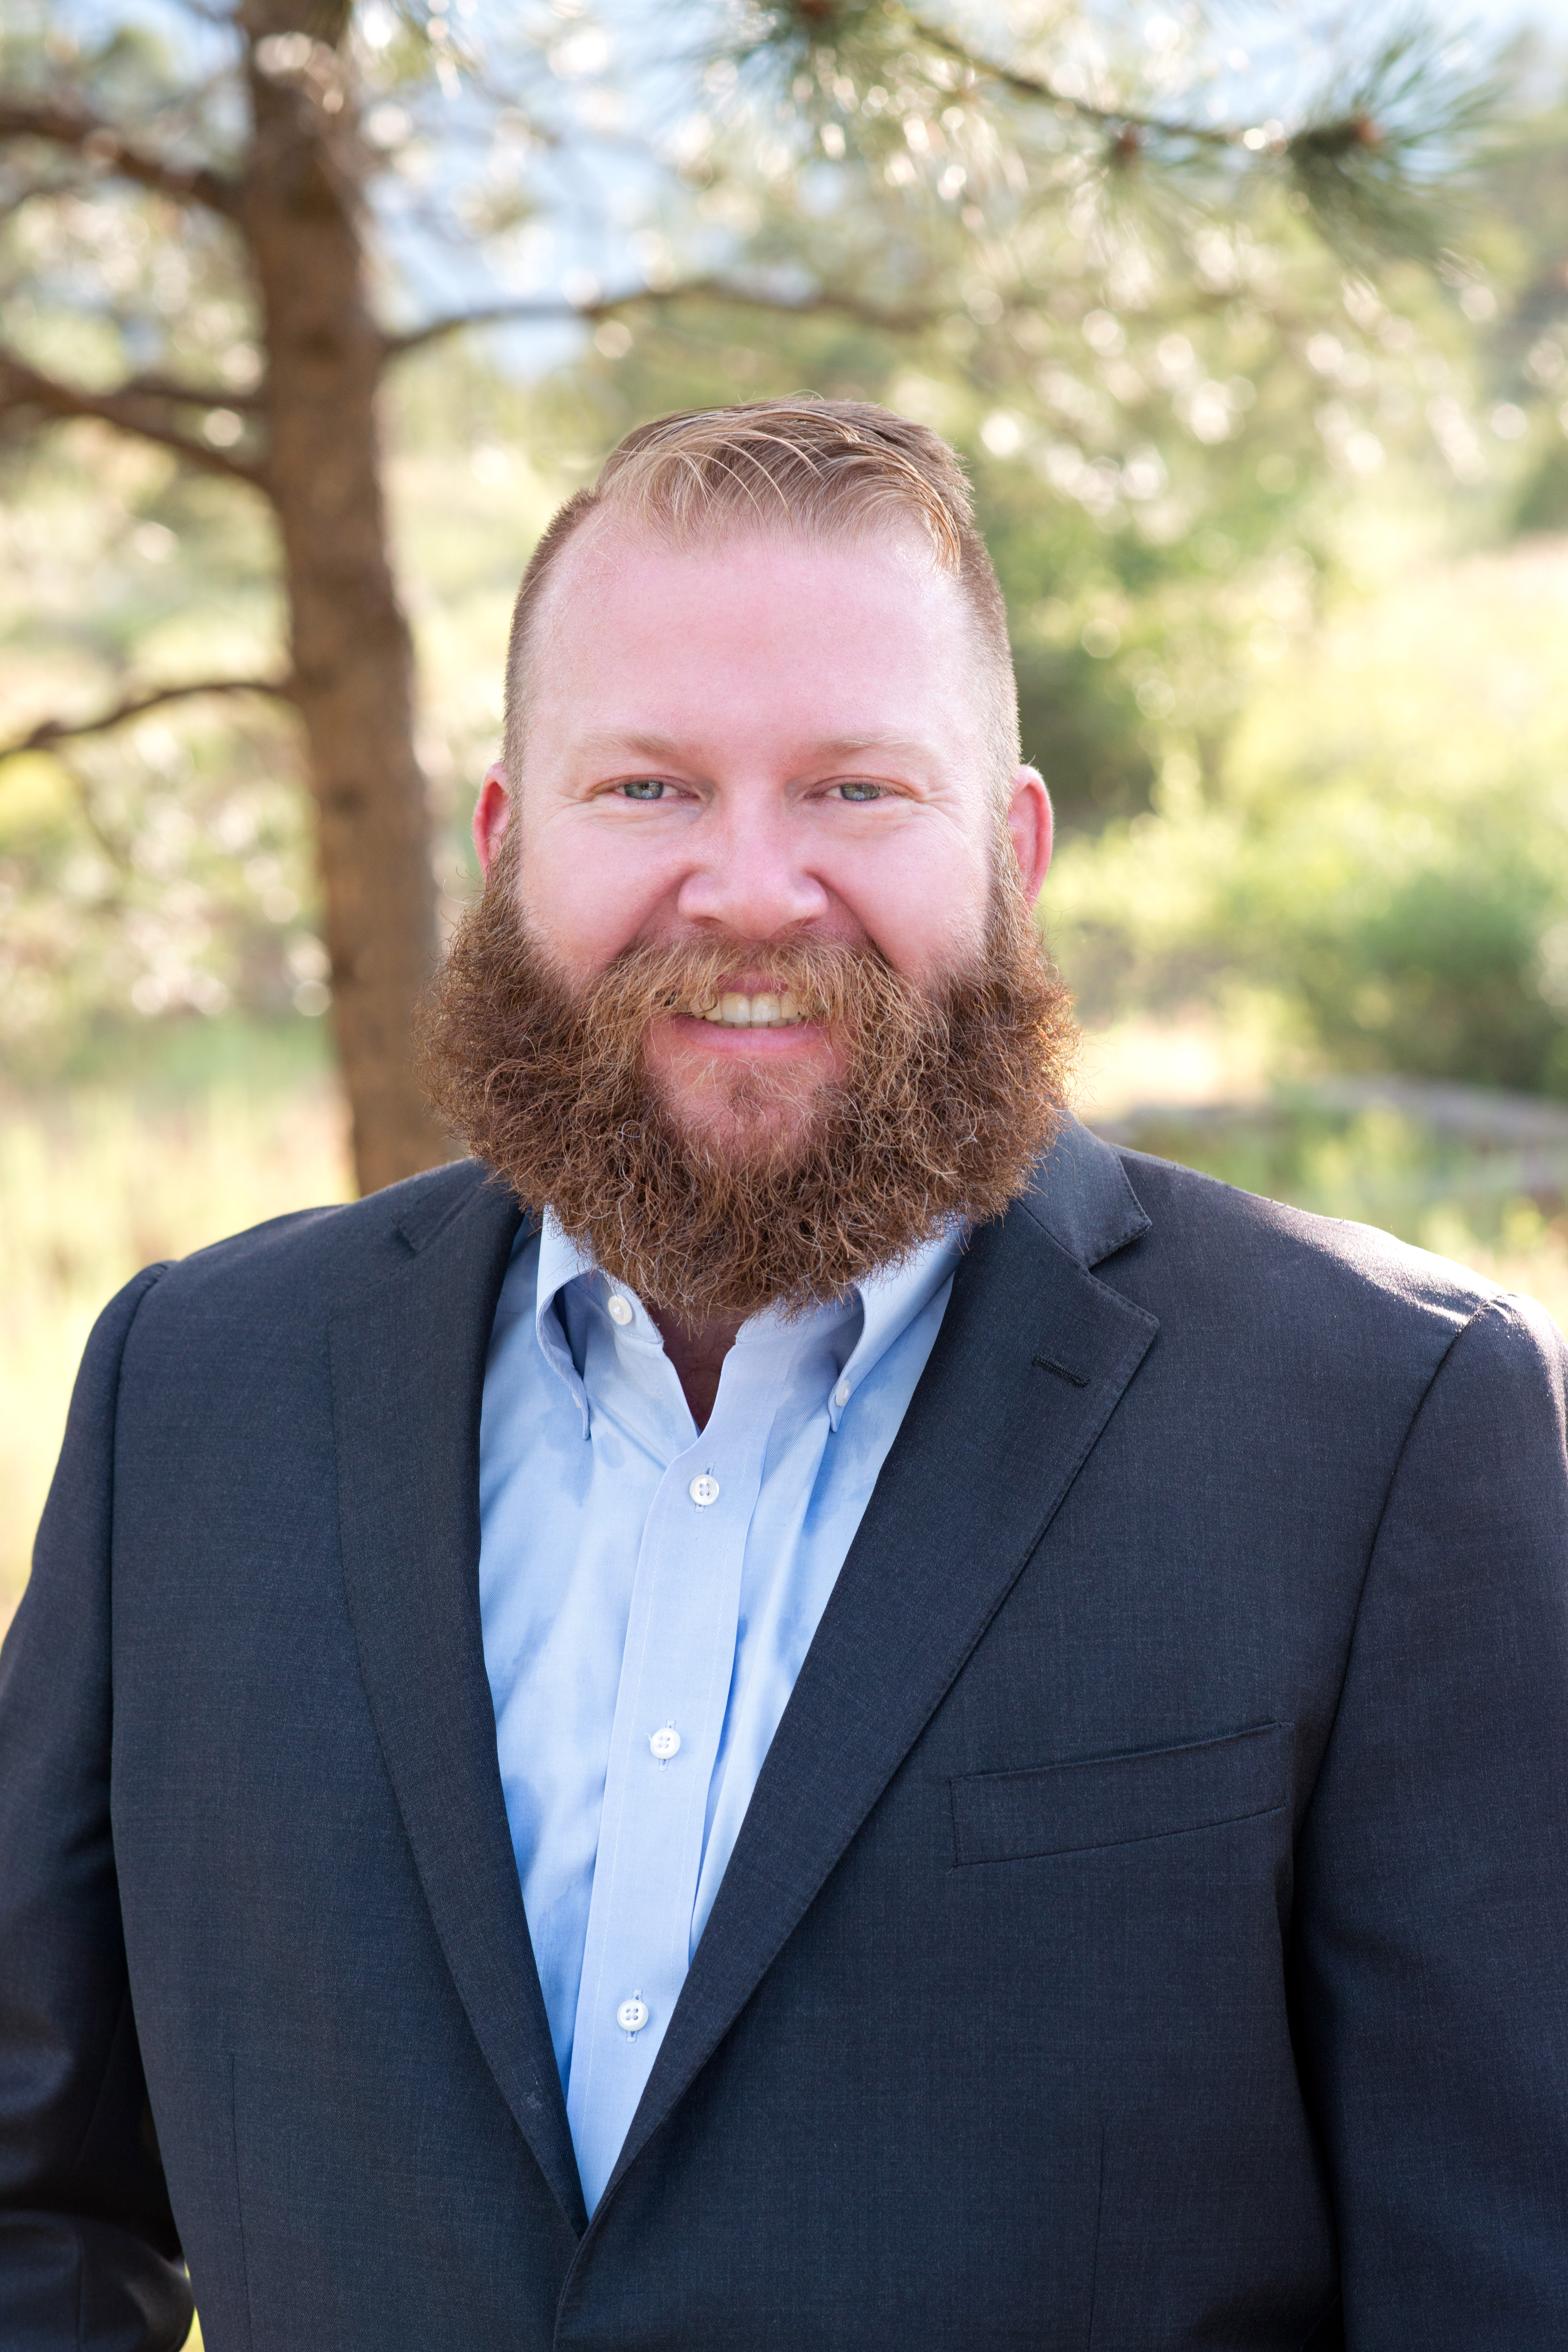
\includegraphics[width=50mm]{headshot.jpg}}
  \caption{Rodger Byrd}
  \label{fig:HS}
\end{figure} 
I work full time for an engineering consulting firm in the field of cybersecurity. My main motivation for graduate school was to become credentialed in the specific field that I've been working in since I completed my Bachelor's Degree. I would also like to open up more career options. I have two young children and with career, my available free time is constrained, so the decision to pursure more education after I complete my Master's Degree is a difficult one. I'm hoping this course will help to inform that decision. I've included a picture of myself above in figure \ref{fig:HS}.

\section{Git Repository}
The files for this latex document are in the github repository located at \path{https://github.com/rodger79/CS6000}. I used Texmaker and BibTeX to build the pdf from the latex project files.

The first problem I encountered was getting my latex tool to work with the IEEEtran plugin. I also learned that doing references for 25 papers can be very time consuming. I hadn't used a separate .bib file in a latex project before so that took a little troubleshooting to get to work. I also had to remember how to use math mode in Latex. It's been a while since I've used it.

\section{Research}
I'm particularly interested in anti-patterns in code so most of the papers I found were related to that field. 

The first of the five papers I read was about very small patterns in source code and how they can be used to identify potential vulnerabilites in the code. The authors\cite{7} referred to these as micro or nano patterns. Nano patterns were defined as a method level pattern and they showed that they could better predict vulnerable methods in code than with software metrics.

The next paper I read looked at anti-patterns in exception handling. They\cite{18}  used data analysis to identify multiple anti-patterns in exception handling that could cause software failures.

The third paper\cite{23} I looked at studied whether software design patterns were actually useful in training new software developers. They claim that novice software developers misuse design patterns, but they didn't have good data to support their claim.

The next paper \cite{25} came up with a technique to use unit testing to identify anti-patterns in code. They came up with a tool to detect known anti patterns in source code. 

The last paper \cite{Carmine} looked at how anti-patterns can redcue the benefits of continuous integration practices. They used the following expression $(\Delta_{Breaks} < 0 ) \wedge (\Delta_{Runs} < 0  \vee \Delta_{Skipped} > 0) $ to determine whether a specific unit test was skipped in a following build.


The other papers are cited in the bibliography. \cite{1} \cite{2} \cite{4} \cite{5} \cite{6}  \cite{8} \cite{9} \cite{10} \cite{11} \cite{12} \cite{13} \cite{14} \cite{15} \cite{16} \cite{17} \cite{19} \cite{20} \cite{21} \cite{22} \cite{23} \cite{24}

\bibliographystyle{IEEEtran}
\bibliography{references}


%\begin{thebibliography}{9}
%\bibitem{git} 
%Project github, \\\path{https://github.com/rodger79/CS6000}
%\bibitem{jflap} 
%JFLAP, \\\path{http://www.jflap.org/getjflap.html}
%\end{thebibliography}

\end{document}